\documentclass[10pt,UTF8]{ctexart}


\usepackage[margin=2cm,a4paper]{geometry}
%\usepackage[left=0.75in,top=0.6in,right=0.75in,bottom=1.0in,a4paper]{geometry}

\setmainfont{Caladea}
%% 也可以選用其它字庫:
% \setCJKmainfont[%
%   ItalicFont=AR PL KaitiM GB,
%   BoldFont=Noto Sans CJK SC,
% ]{Noto Serif CJK SC}
% \setCJKsansfont{Noto Sans CJK SC}
% \renewcommand{\kaishu}{\CJKfontspec{AR PL KaitiM GB}}

% 繁體中文
\setCJKmainfont[Path=fonts/ ]{NotoSansTC-Medium.otf}

\usepackage{minted}
\usepackage[breaklinks]{hyperref}

% Picture
% 導言區的此三行無變化
\usepackage{graphicx}
\usepackage{float} 
\usepackage{subfigure}
% 以下是新增的自定義格式更改
\usepackage[]{caption2} %新增調用的宏包
\renewcommand{\figurename}{Fig.} %重定義編號前綴詞
\renewcommand{\captionlabeldelim}{.~} %重定義分隔符
 %\roman 是羅馬數字編號,\alph是默認的字母編號,\arabic是阿拉伯數字編號,可按需替換下一行的相應位置
\renewcommand{\thesubfigure}{(\roman{subfigure})}%此外,還可設置圖編號顯示格式,加括號或者不加括號
\makeatletter \renewcommand{\@thesubfigure}{\thesubfigure \space}%子圖編號與名稱的間隔設置
\renewcommand{\p@subfigure}{} \makeatother

% Math
\usepackage {mathtools}
\usepackage{amssymb}

% Code
\usepackage{listings}
\usepackage{xcolor}
\lstset{
    % backgroundcolor=\color{red!50!green!50!blue!50},
    % 程式碼塊背景色為淺灰色
    rulesepcolor= \color{gray}, % 程式碼塊邊框顏色
    breaklines=true,  % 程式碼過長則換行
    numbers=left, % 行號在左側顯示
    numberstyle= \small,% 行號字型
    % eywordstyle= \color{red,% 關鍵字顏色
    commentstyle=\color{gray}, % 註釋顏色
    frame=shadowbox % 用方框框住程式碼塊
    }

\usepackage{hyperref}

\title{數字媒體軟件與系統開發}
\author{干皓丞,2101212850, 信息工程學院}

\begin{document}
\maketitle


\section{作業目標與章節摘要}

利用 live555 和 VLC 播放器,搭建一个流媒体播放系统。

\begin{figure}[H]
\centering 
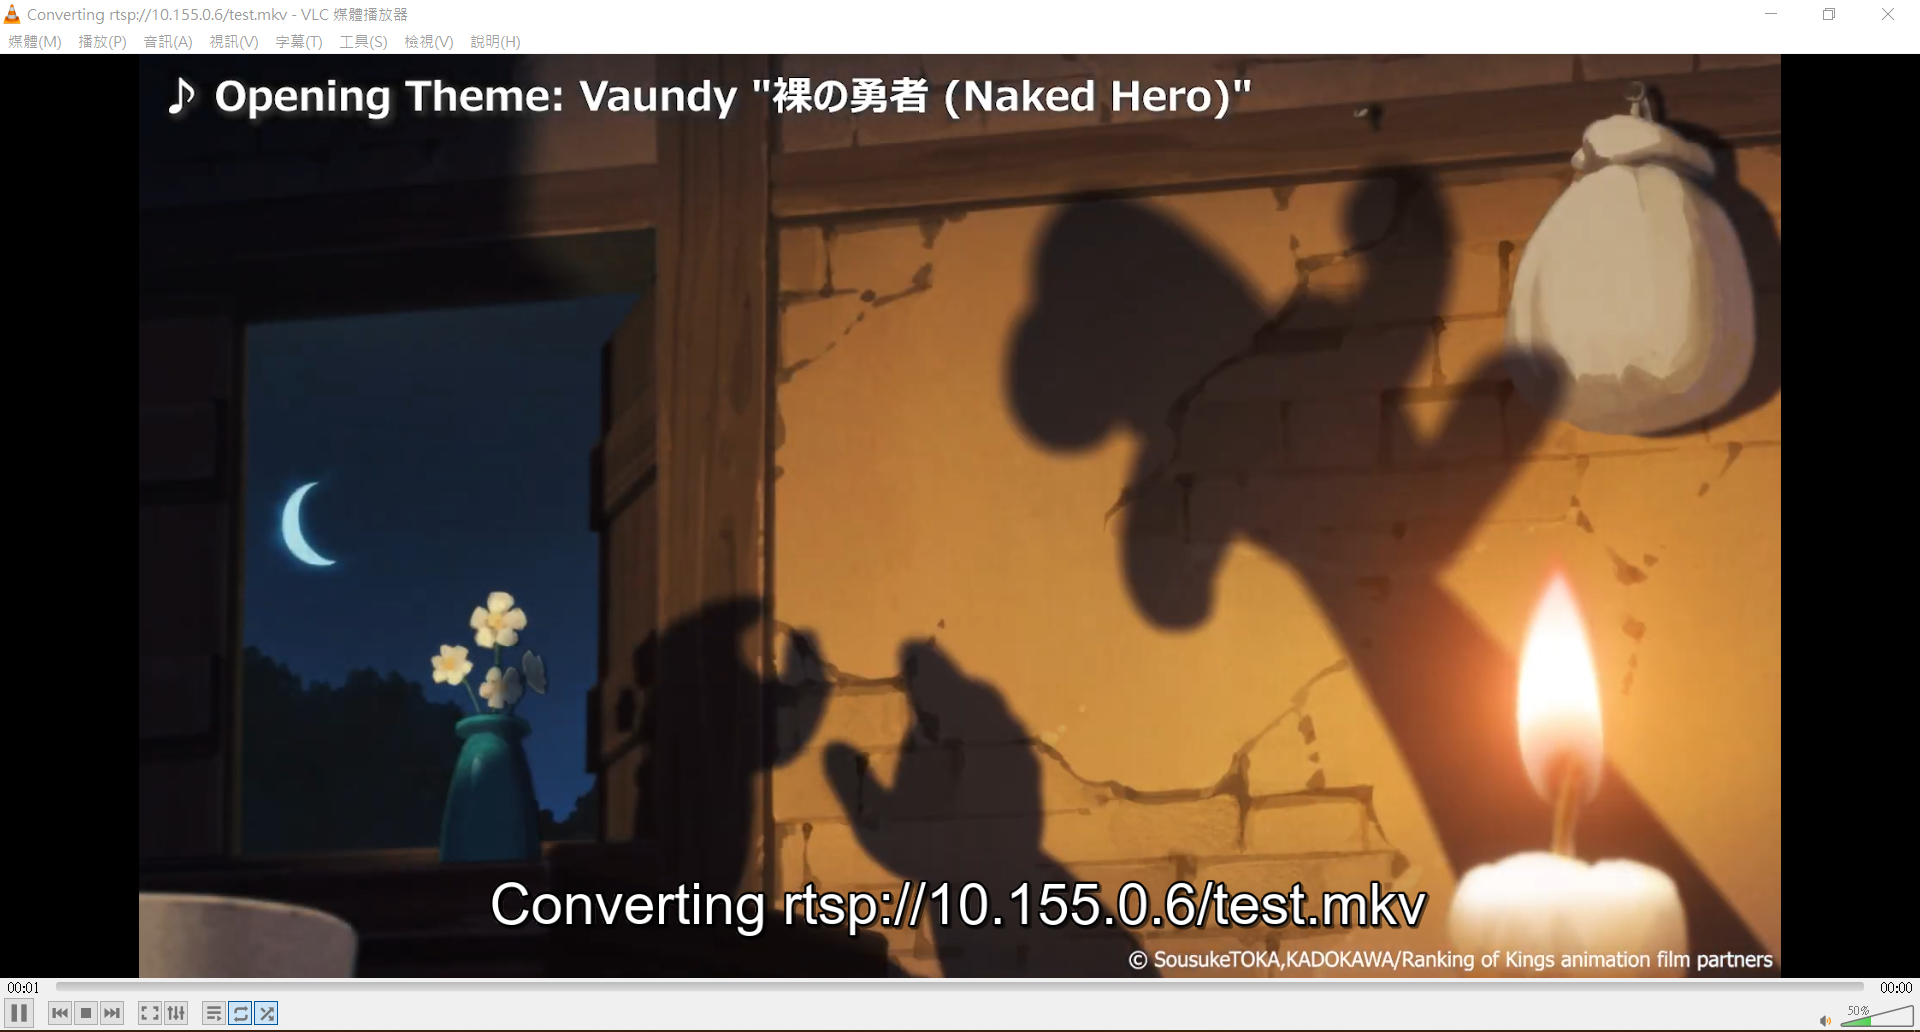
\includegraphics[width=0.80\textwidth]{13.png} 
\caption{Live555 和 VLC 作業完成畫面}
\label{Test}
\end{figure}

\begin{figure}[H]
\centering 
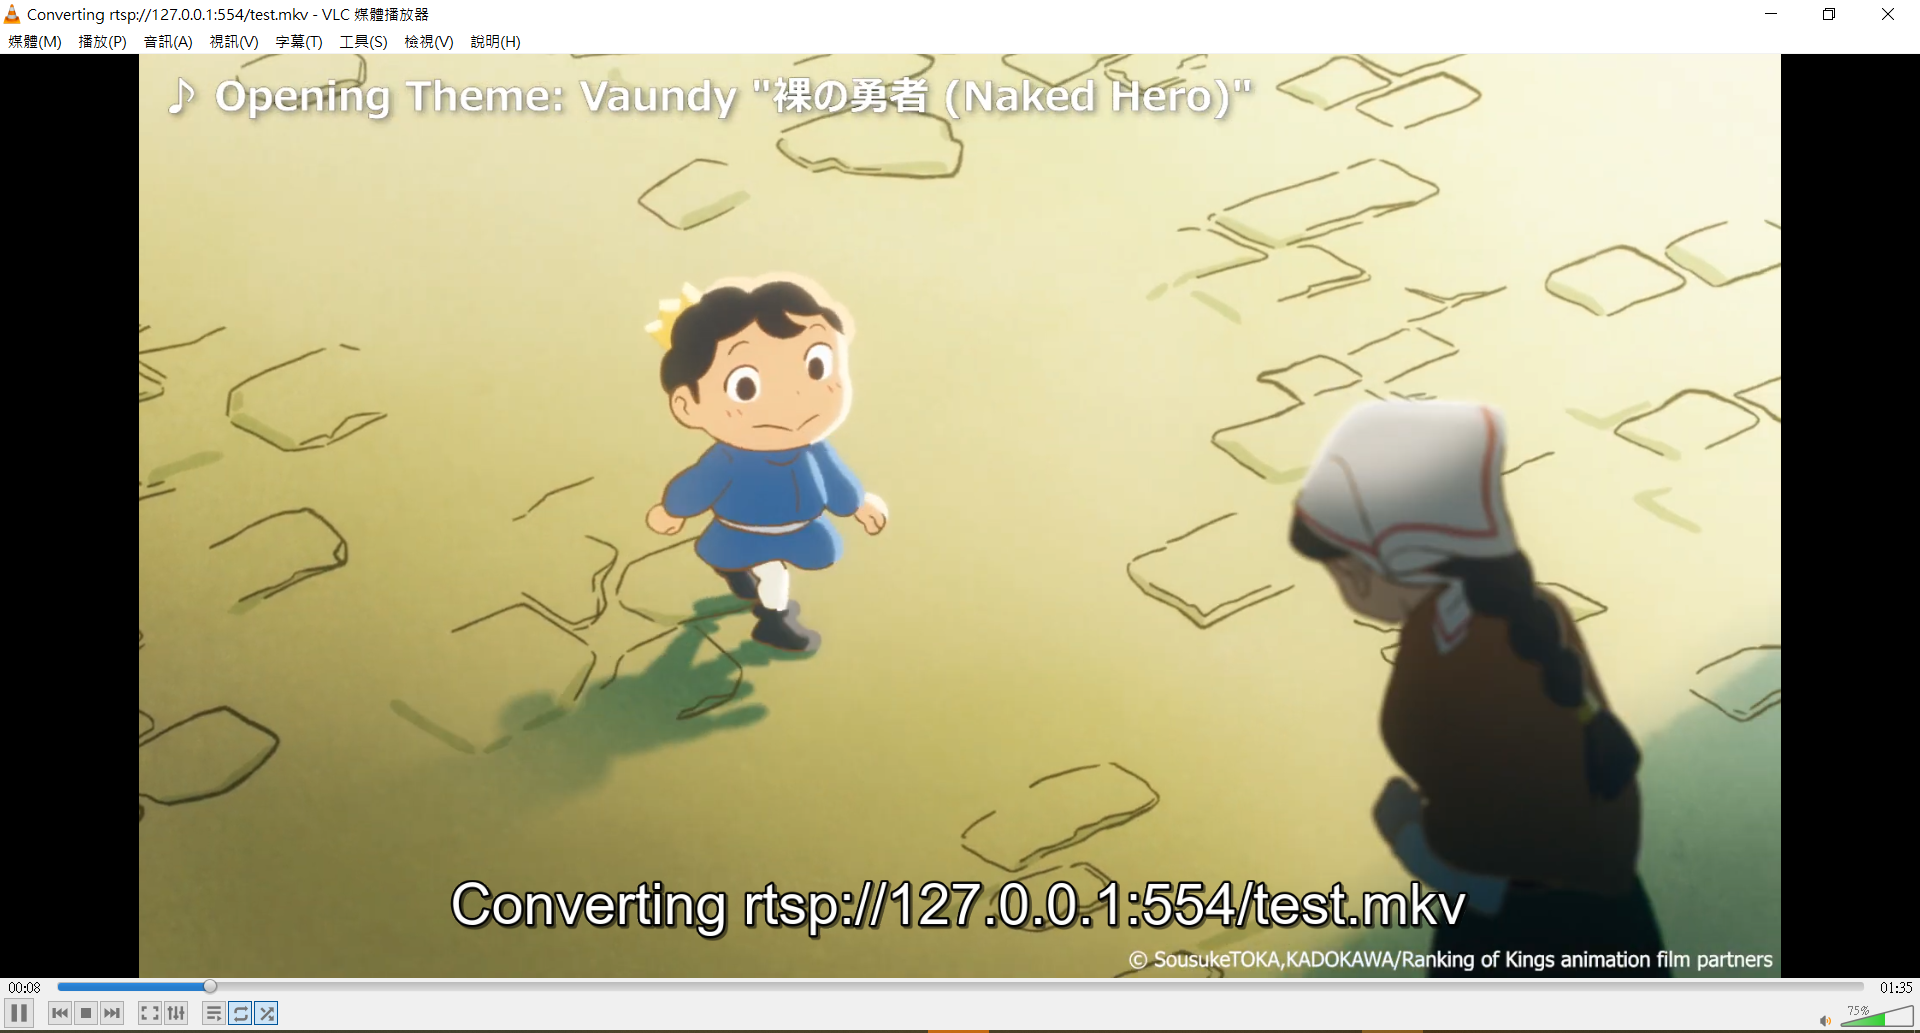
\includegraphics[width=0.80\textwidth]{17.png} 
\caption{Live555 和 VLC  Docker 版本的作業完成畫面}
\label{Test}
\end{figure}


\section{文章與作業狀況}

作業可以從 GitHub 下的 kancheng/kan-cs-report-in-2022 專案找到,作業程式碼與文件目錄為 kan-cs-report-in-2022/DMSASD/live5552vlc。實際執行的環境與實驗設備為 Google 的 Colab 、MacBook Pro (Retina, 15-inch, Mid 2014) 、 Acer Aspire R7 與 HP Victus (Nvidia GeForce RTX 3060)。


\section{作業內容概述}

此作業分三大部分,第一部分說明 Live555 與 VLC 撥放器,第二部分 Live555 在 Windows 編譯、架設 Server 與 VLC 設定,而第三部分 Docker 的 Live555 架設 Server 與 VLC 設定,最後則是錯誤紀錄。而本次測試影像則是源自於動畫國王排名的開頭影像,由 Ani-One 代理於 YOUTUBE 地區頻道。

1. Live555 與 VLC 撥放器說明

2. Live555 在 Windows 編譯、架設 Server 與 VLC 設定

3. Docker 的 Live555 架設 Server 與 VLC 設定

4. 額外紀錄

\begin{figure}[H]
\centering 
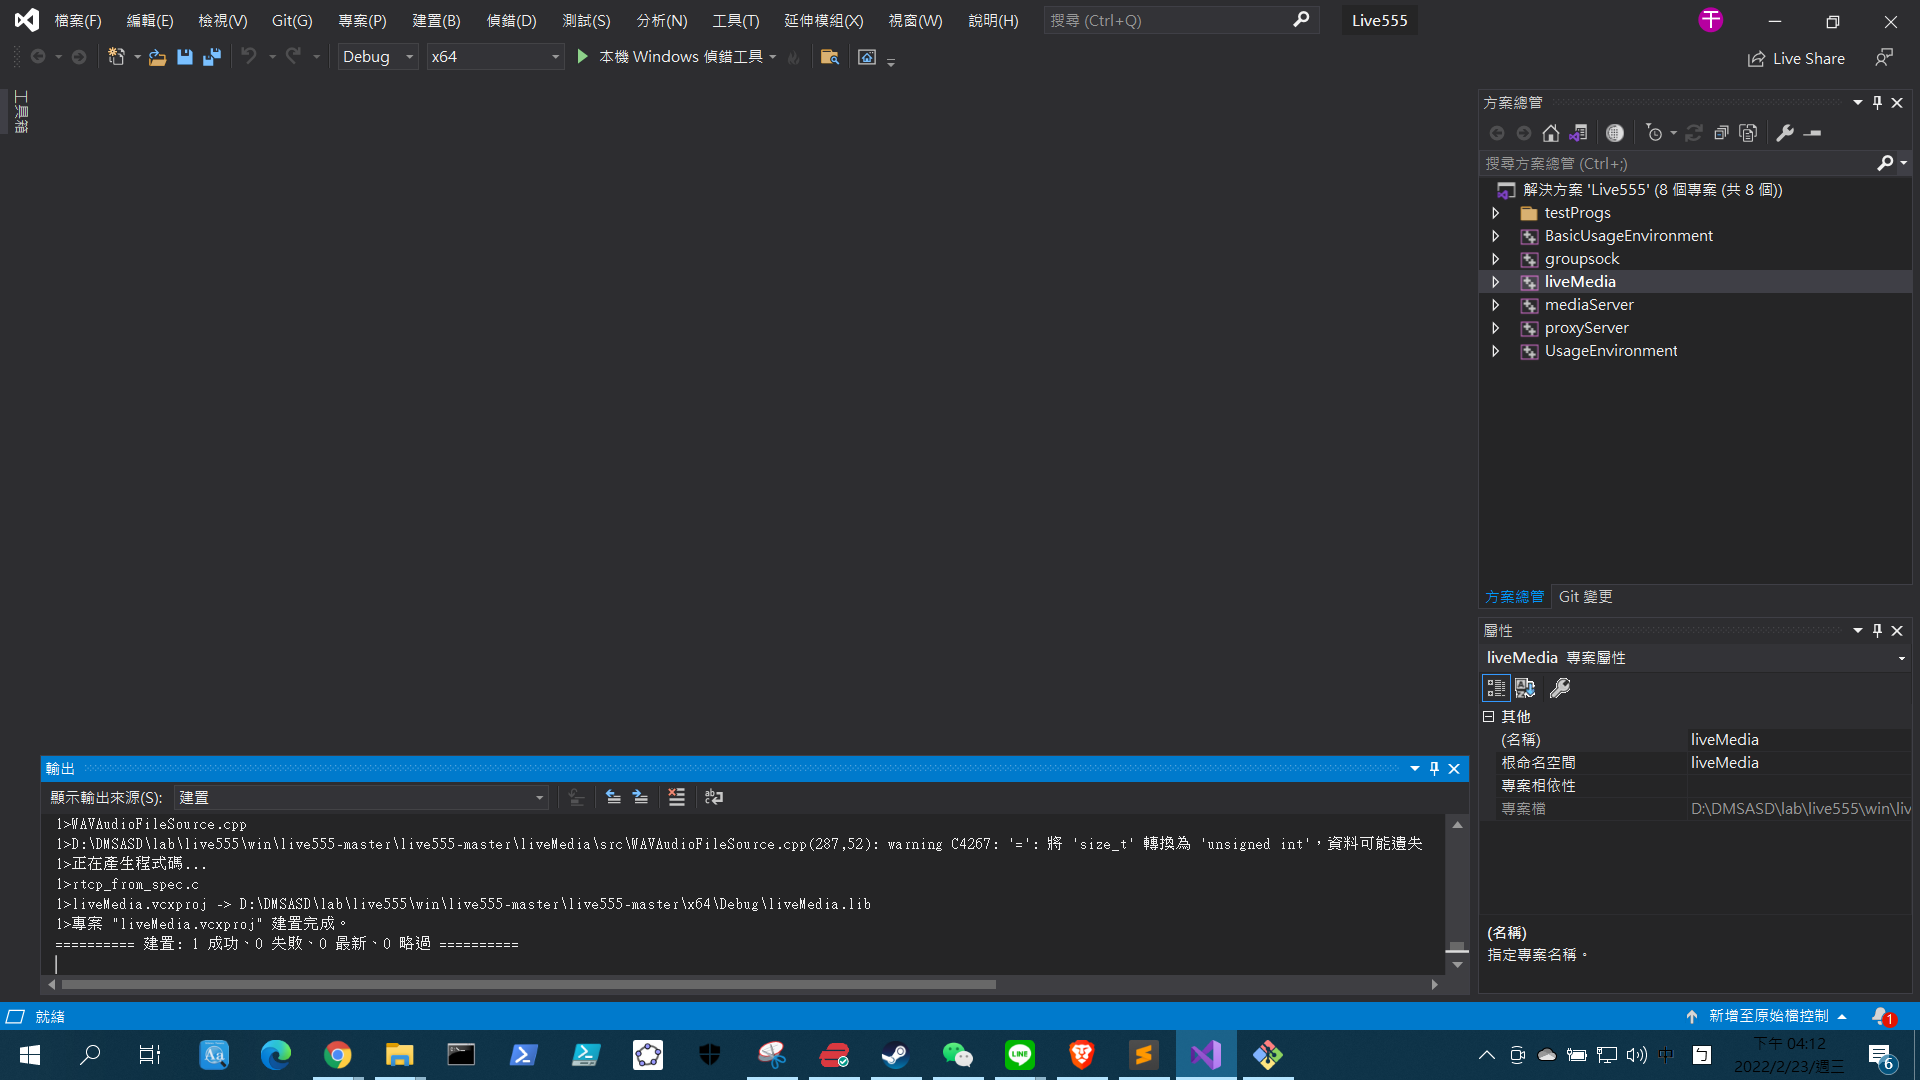
\includegraphics[width=0.80\textwidth]{1.png} 
\caption{Live555 編譯}
\label{Test}
\end{figure}


\section{Live555 與 VLC 撥放器說明}

Live555 流媒體是由 Live Networks, Inc. 所開發的一組開源(LGPL) C++ 庫,用於多媒體流媒體。而該庫支持流式傳輸的 RTP / RTCP 和 RTSP 等開放標準,還可以管理 H.264、H.265、MPEG、VP8 和 DV 等視頻。而本作業的所編譯 Live555 的專案來源為 cmberryau/live555。而 VLC 則是多媒體播放器 為 VideoLAN 所規劃的開放原始碼的專案,該專案支援眾多音訊與影像解碼器跟檔案格式,並支援 DVD 影音光碟、 VCD 影音光碟等各類串流協定。

\section{Live555 在 Windows 編譯、架設 Server 與 VLC 設定}

Live555 於專案下載下來後處理錯誤問題,而後從 debug 中取得檔案,將其與測試影像檔案放入同個目錄中執行。

\begin{figure}[H]
\centering 
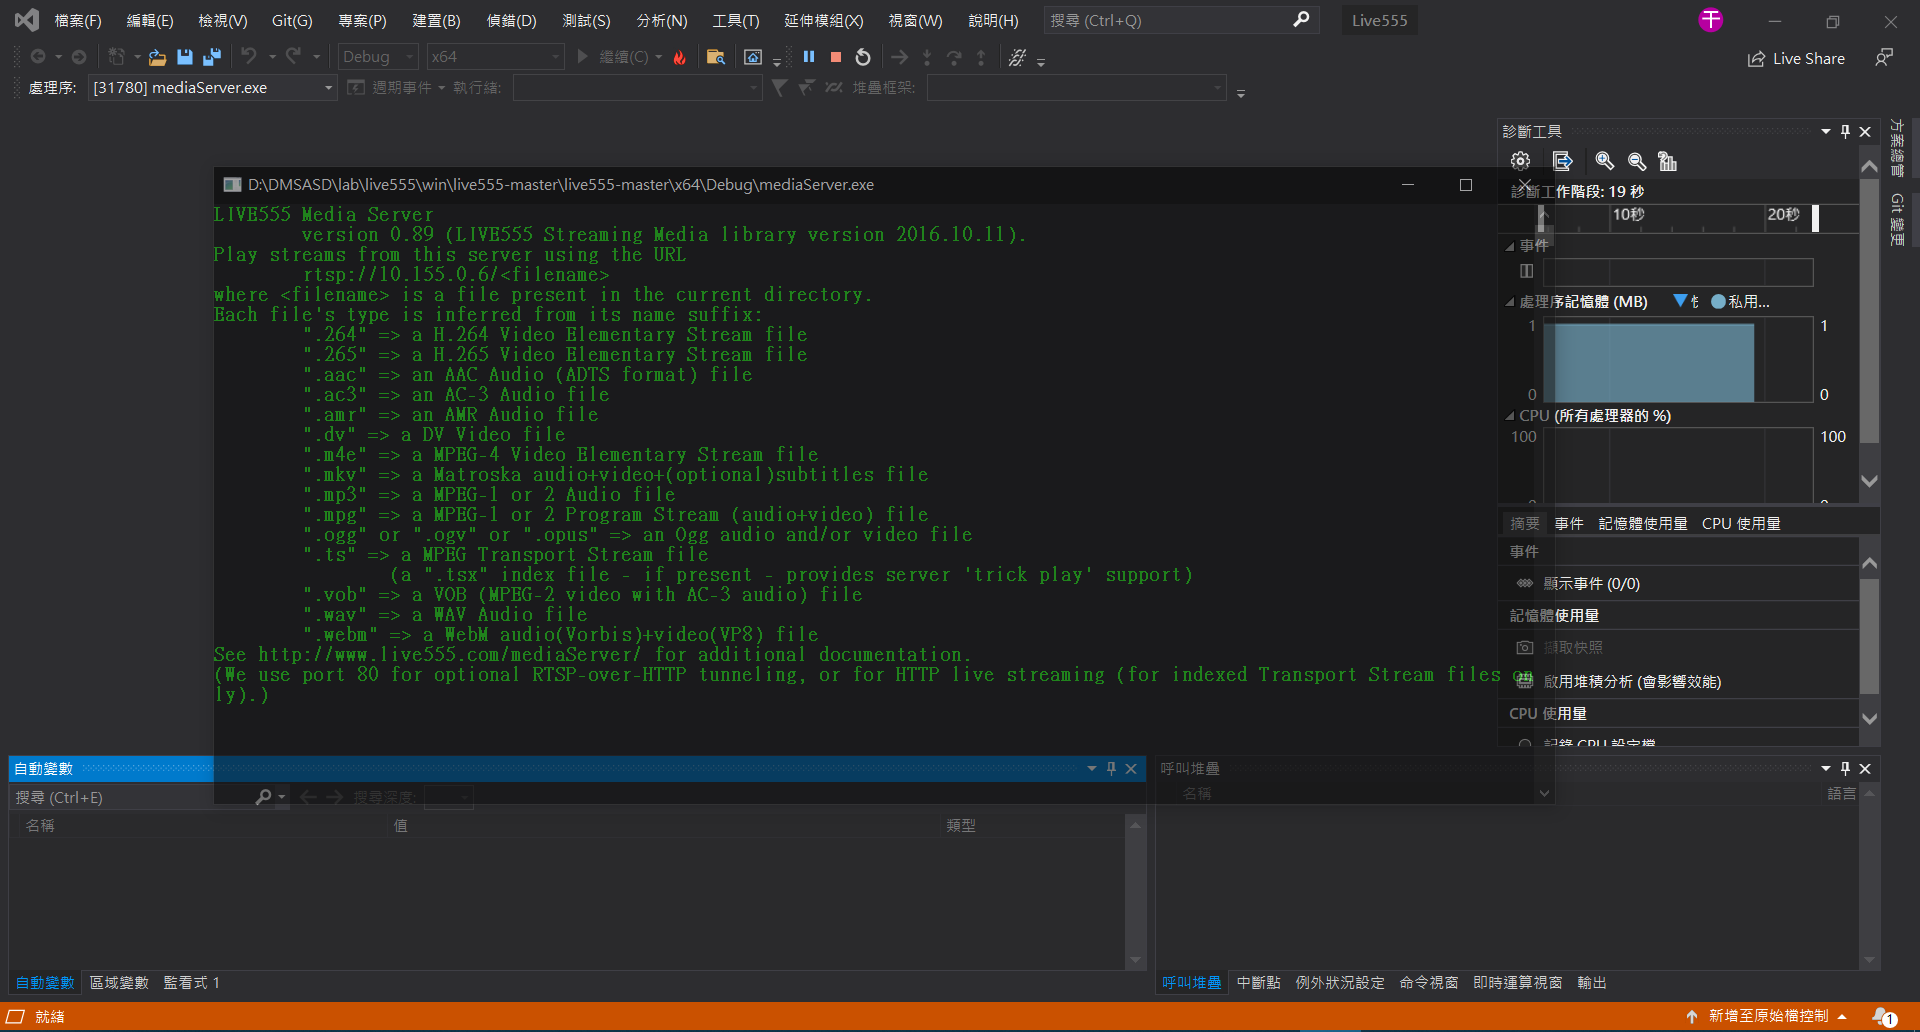
\includegraphics[width=0.80\textwidth]{4.png} 
\caption{Live555 編譯成功}
\label{Test}
\end{figure}

\begin{figure}[H]
\centering 
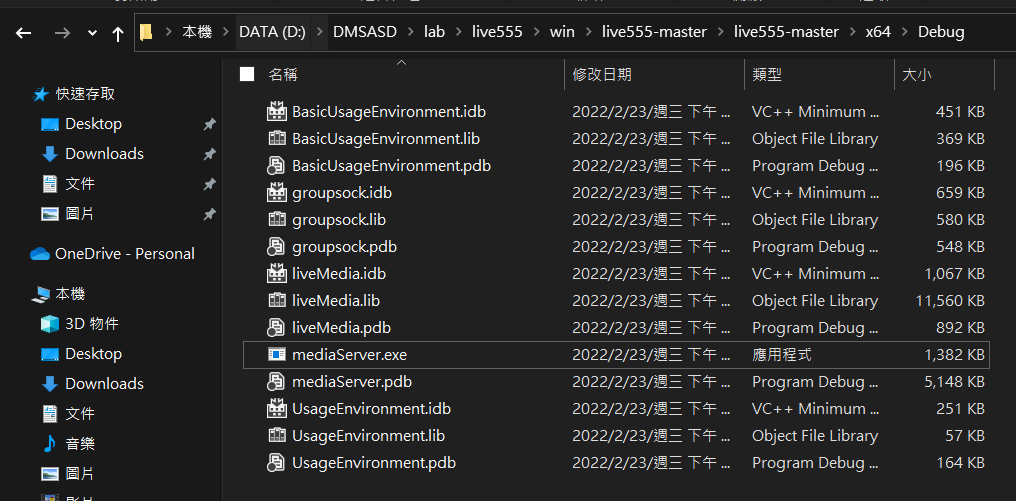
\includegraphics[width=0.80\textwidth]{5.png} 
\caption{mediaServer 的 exe 檔案}
\label{Test}
\end{figure}

\begin{figure}[H]
\centering 
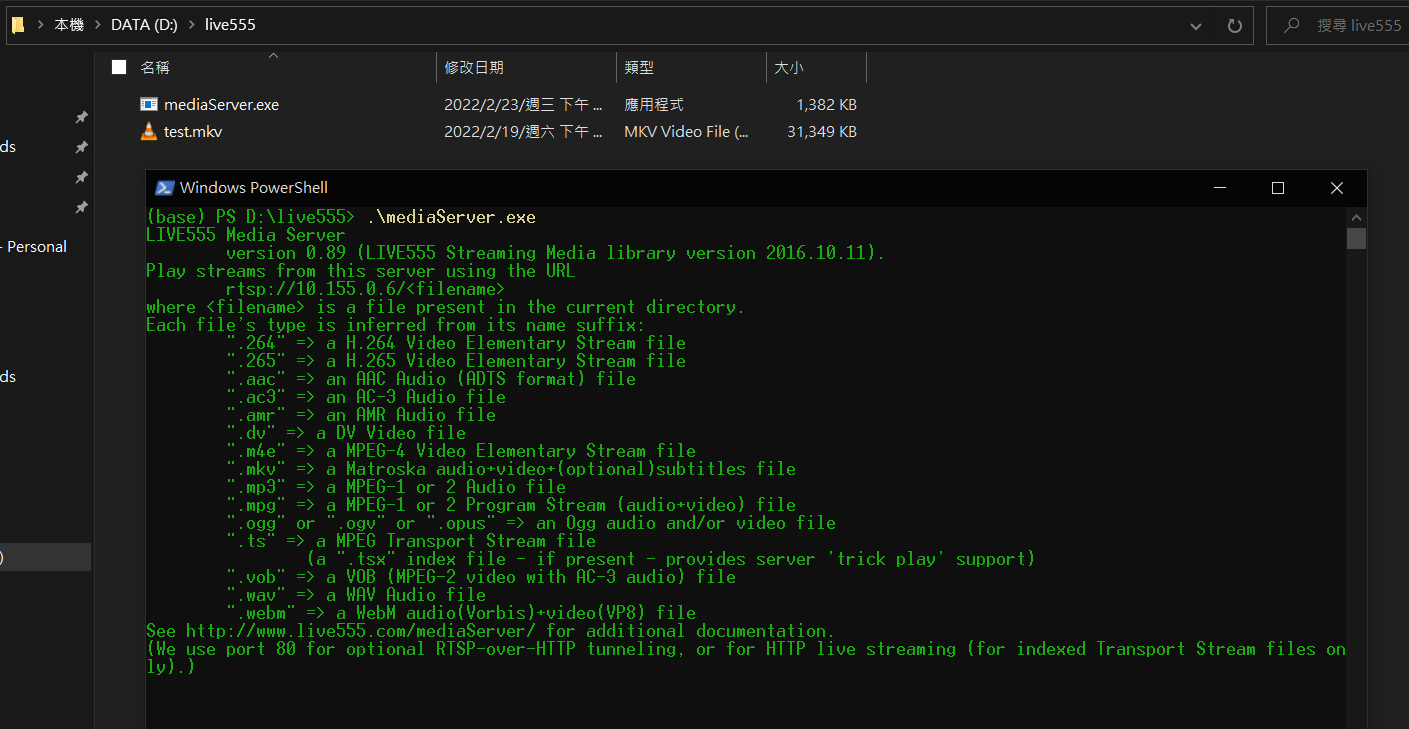
\includegraphics[width=0.80\textwidth]{6.png} 
\caption{Server 執行}
\label{Test}
\end{figure}

根據 Server 執行的資訊來設定 VLC。在此步驟如下。

\begin{figure}[H]
\centering 
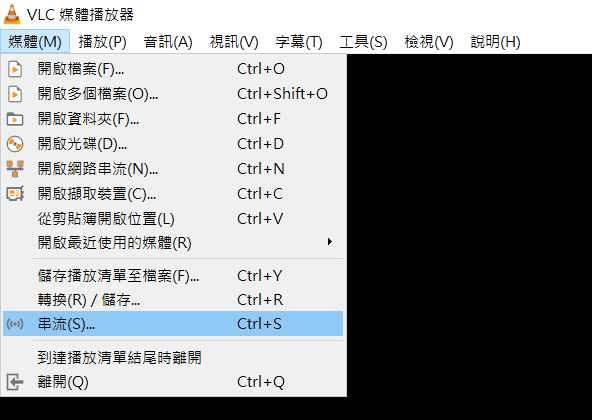
\includegraphics[width=0.80\textwidth]{7.png} 
\caption{按下串流}
\label{Test}
\end{figure}

\begin{figure}[H]
\centering 
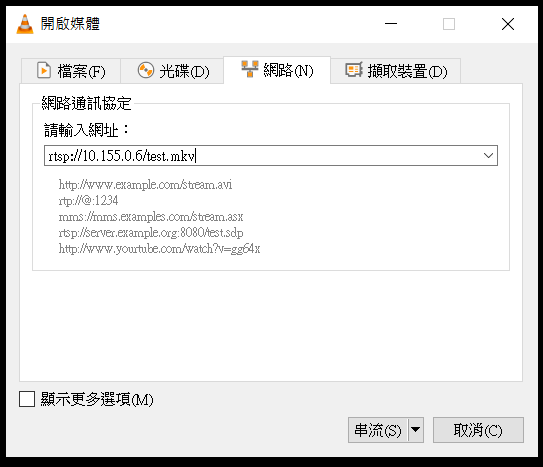
\includegraphics[width=0.80\textwidth]{8.png} 
\caption{選擇網路}
\label{Test}
\end{figure}

\begin{figure}[H]
\centering 
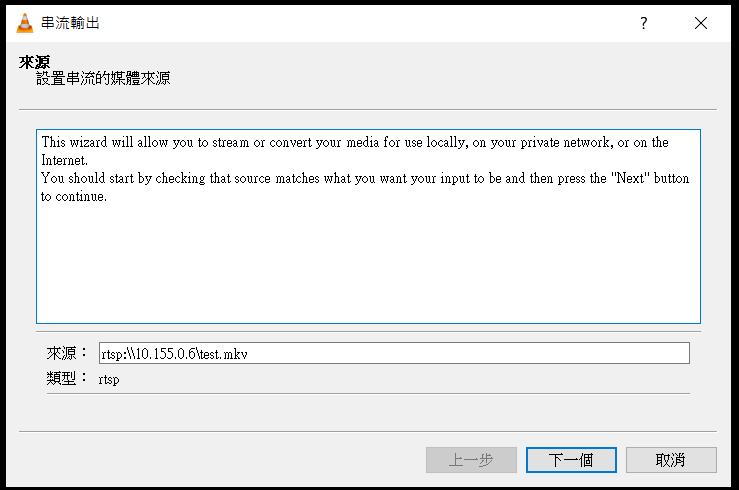
\includegraphics[width=0.80\textwidth]{9.png} 
\caption{來源}
\label{Test}
\end{figure}

\begin{figure}[H]
\centering 
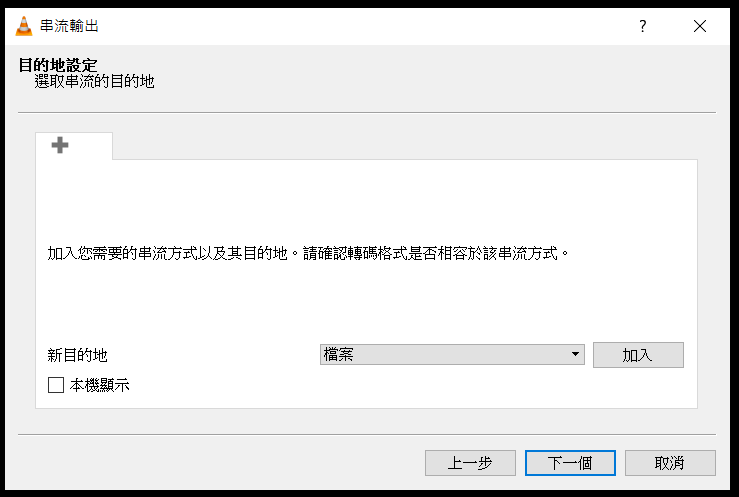
\includegraphics[width=0.80\textwidth]{10.png} 
\caption{可設定目的地}
\label{Test}
\end{figure}

\begin{figure}[H]
\centering 
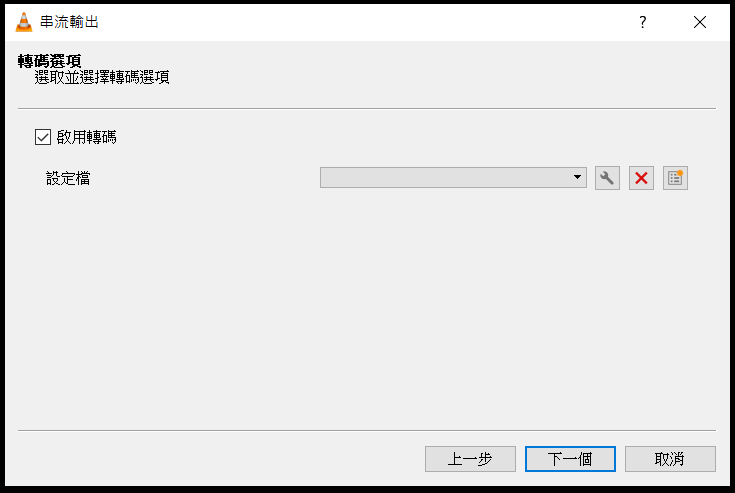
\includegraphics[width=0.80\textwidth]{11.png} 
\caption{轉碼}
\label{Test}
\end{figure}

\begin{figure}[H]
\centering 
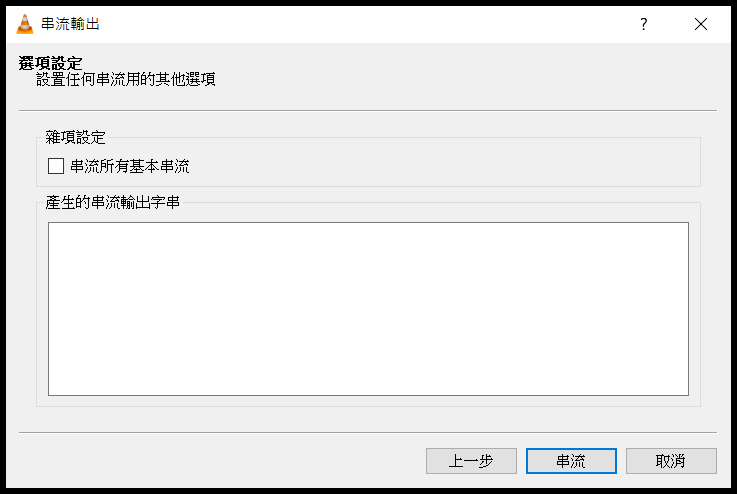
\includegraphics[width=0.80\textwidth]{12.png} 
\caption{雜項}
\label{Test}
\end{figure}

\begin{figure}[H]
\centering 
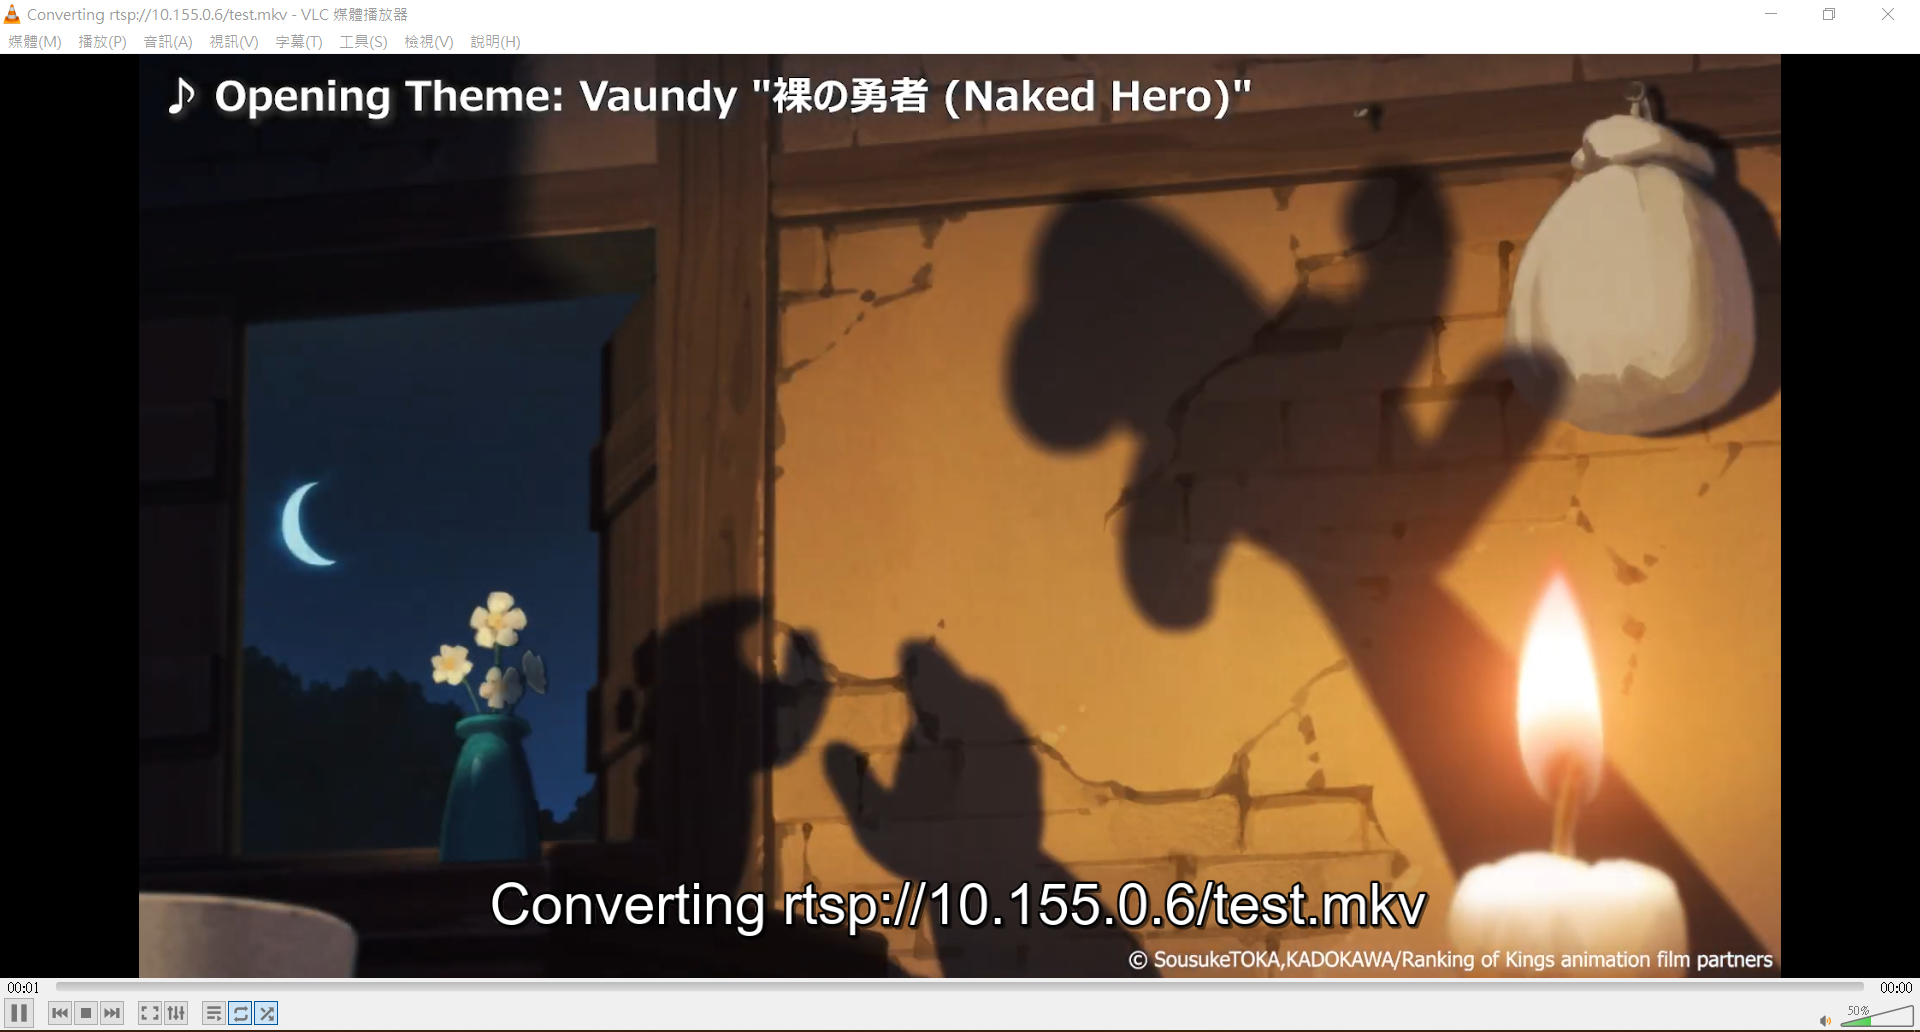
\includegraphics[width=0.80\textwidth]{13.png} 
\caption{完成}
\label{Test}
\end{figure}

\section{Docker 的 Live555 架設 Server 與 VLC 設定}

在此的 Docker 版本與前者類似,前提條件是 WSL 等環境要事先準備好。拉下指定的映象檔案即可,最後執行並設定 VLC。

\begin{lstlisting}[language={python}]
docker pull vimagick/live555

docker run -p 9488:87 -p 554:554 -it -v D:\docker-save\live555-server:/data vimagick/live555 /bin/bash

\end{lstlisting}

\begin{figure}[H]
\centering 
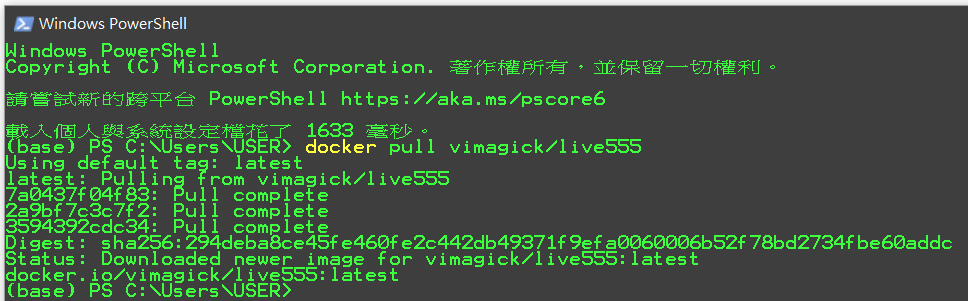
\includegraphics[width=0.80\textwidth]{14.png} 
\caption{拉映像檔}
\label{Test}
\end{figure}

\begin{figure}[H]
\centering 
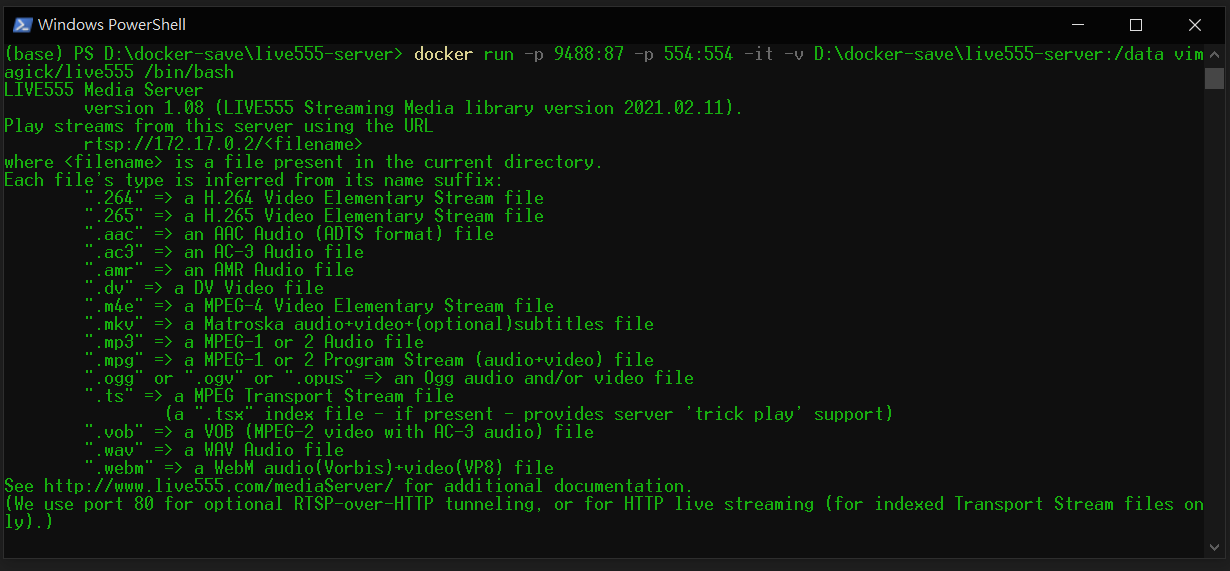
\includegraphics[width=0.80\textwidth]{15.png} 
\caption{執行容器}
\label{Test}
\end{figure}

\begin{figure}[H]
\centering 
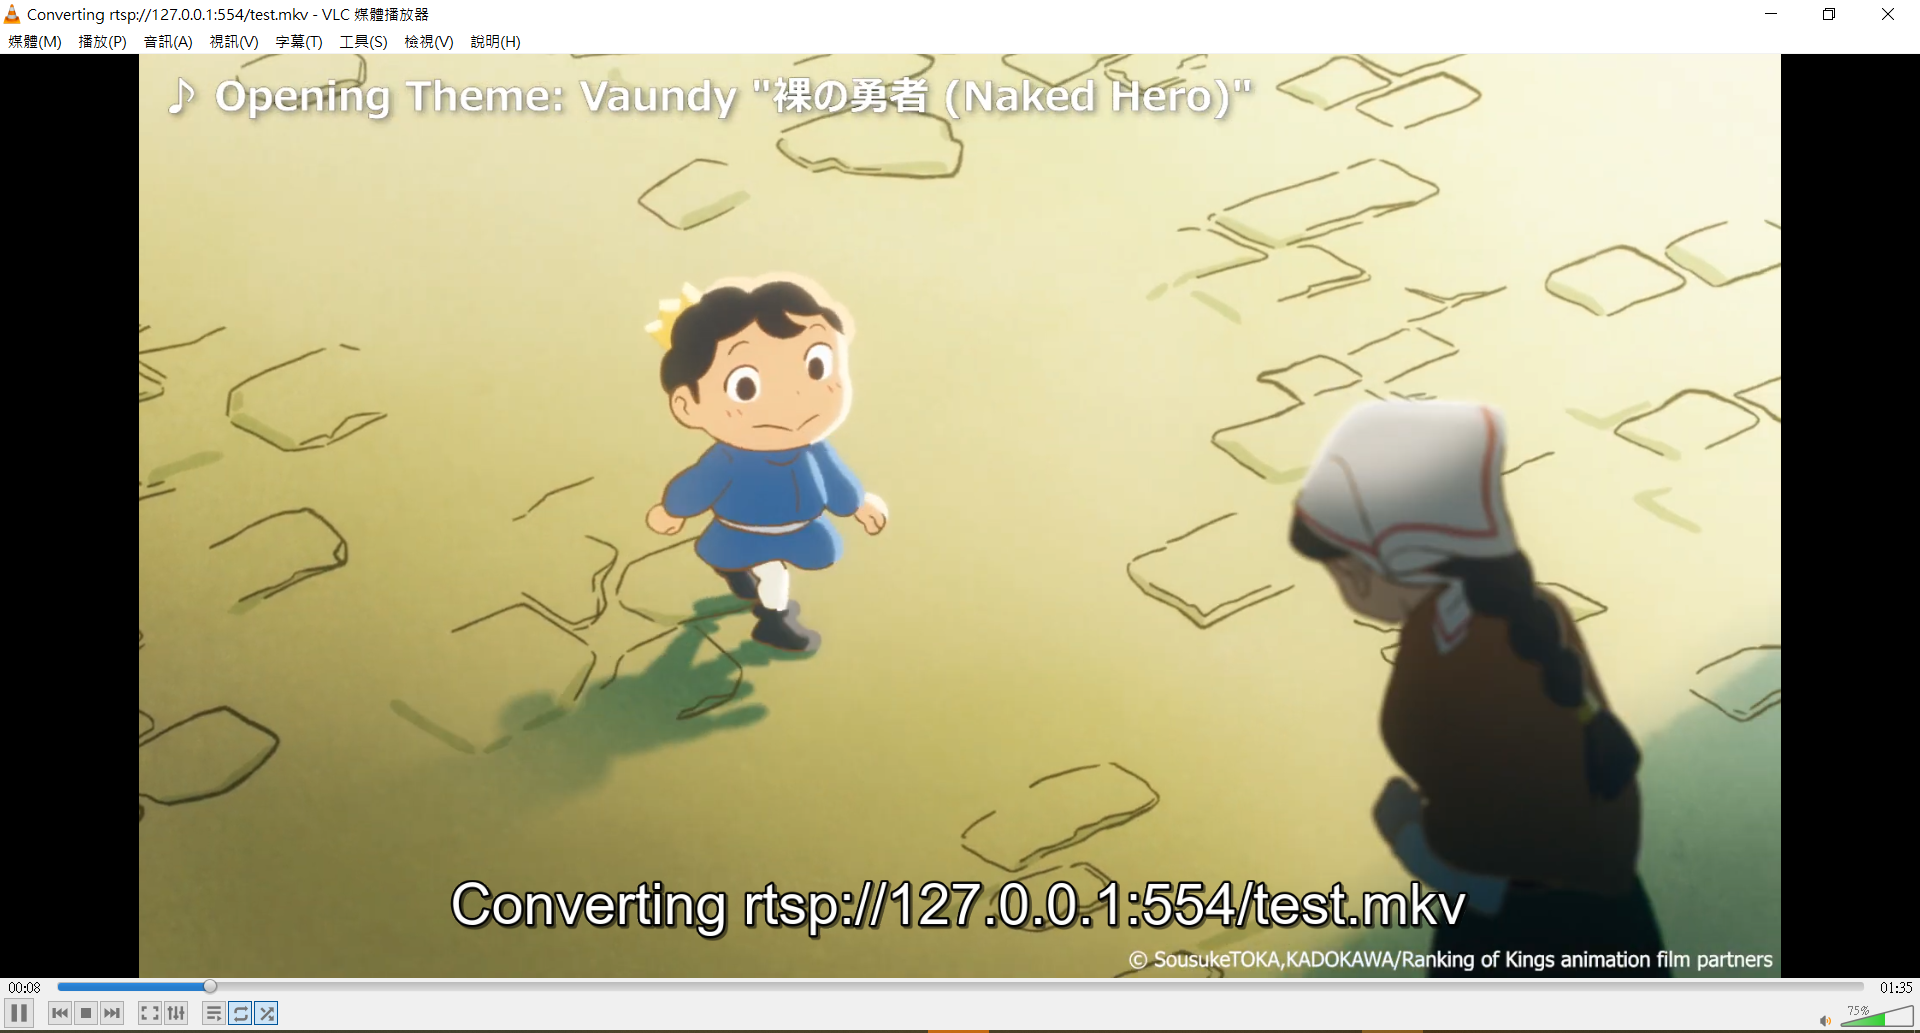
\includegraphics[width=0.80\textwidth]{17.png} 
\caption{完成}
\label{Test}
\end{figure}

\section{額外紀錄}

Live555 在使用 Visual Studio 2019 編譯時,有面對 liveMedia.lib 不是有效的應用程式的問題等訊息,導致無法順利編譯。而該問題的解決方案是將專案目錄的 mediaServer 目錄設定為啟動專案。

\begin{figure}[H]
\centering 
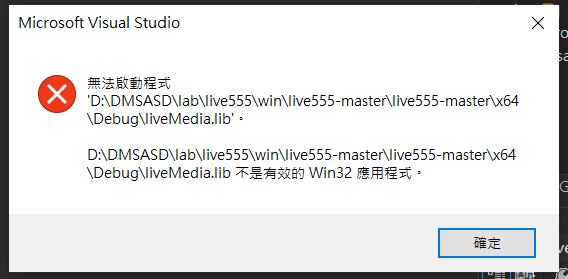
\includegraphics[width=0.50\textwidth]{2.png} 
\caption{Live555 錯誤訊息}
\label{Test}
\end{figure}

\begin{figure}[H]
\centering 
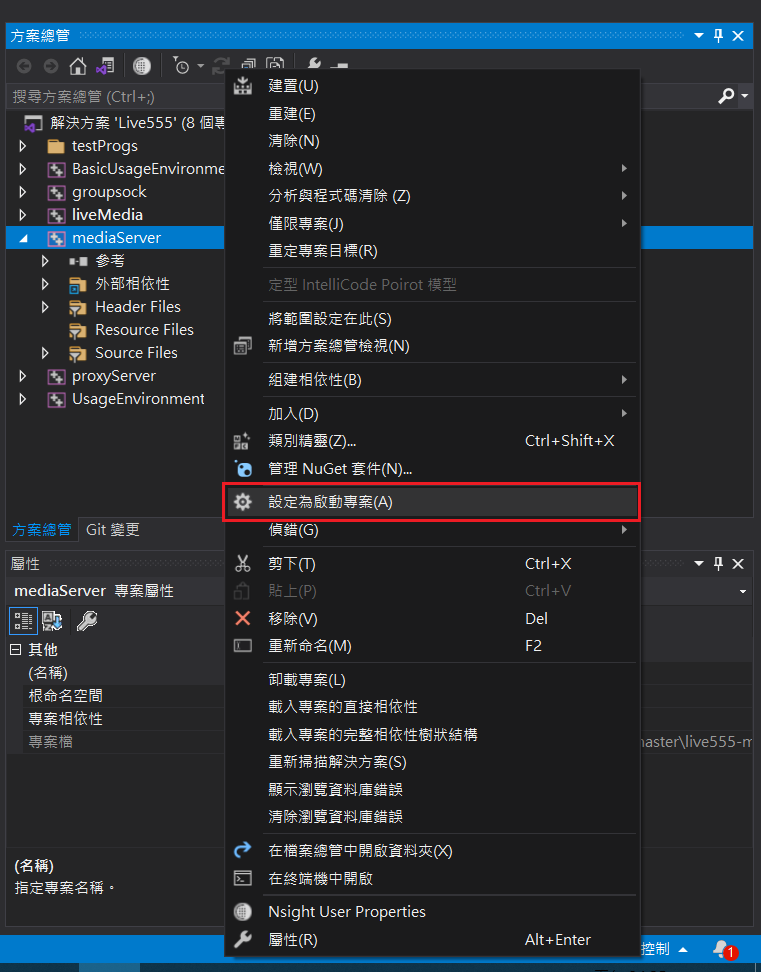
\includegraphics[width=0.80\textwidth]{3.png} 
\caption{Live555 設定為啟動專案}
\label{Test}
\end{figure}

%\section{附錄}

% 數學意義說明

% $$\min \limits_{G}\max \limits_{D}{V_I(D,\ G)=V(D,G)-\lambda L_I(G,Q)}$$

%	\begin{lstlisting}[language={python}]

%	\end{lstlisting}

%\begin{enumerate}
%\item Y
%\item A
%\end{enumerate}

% \newpage

\clearpage

\end{document}